\documentclass[twocolumn,superscriptaddress,aps]{revtex4-1}

\usepackage[utf8]{inputenc}

\usepackage{amsfonts}
\usepackage{amssymb}
\usepackage{amsmath}
\usepackage{amsthm}

\usepackage{bbold}
\usepackage{bm}
\usepackage{graphicx}
\usepackage{color}
\usepackage{hyperref}

\begin{document}


% ==============================================================================

\title{\Large{INFO8010: Interior Design Style Transfer}}
\vspace{1cm}
\author{\small{\bf Marie Goffin}}
\affiliation{\texttt{mgoffin@student.uliege.be} (\texttt{s191956})}
\author{\small{\bf Thomas Fredrich}}
\affiliation{\texttt{thomas.fredrich@student.uliege.be} (\texttt{s191717})}

\maketitle

% ==============================================================================

\section{Introduction}

Interior design visualization remains challenging for non-professionals. Most people struggle to imagine how their spaces would look in different design styles. Traditional visualization methods require either professional design skills or extensive photo editing expertise.\\

In this paper, we explore a machine learning approach for transforming room interior images between design styles. Our method investigates an enhanced CycleGAN architecture that aims to preserve structural elements while changing aesthetic features.\\

Our work examines:

\begin{itemize}
    \item Adapting CycleGAN for room style transfer
    \item Implementing multi-scale discriminators and improved residual blocks 
    \item Testing a structural preservation loss to maintain architectural elements
    \item Evaluating results using LPIPS and FID metrics
\end{itemize}

We focus specifically on transferring between industrial and scandinavian bathroom styles. Our approach works with unpaired datasets, addressing the practical limitation that paired before/after images of the same room in different styles are rarely available.

\section{Related Work}

\subsection{Image-to-Image Translation}
Image-to-image translation has seen significant progress in recent years. Pix2Pix \cite{isola2017image} introduced a general framework for supervised image translation using conditional GANs, requiring paired training data. CycleGAN \cite{zhu2017unpaired} extended this approach to the unpaired setting by introducing cycle consistency loss, enabling training without directly corresponding before/after images. This unpaired approach is particularly valuable for interior design applications, where obtaining before/after photos of the same room in different styles is difficult.

\subsection{Style Transfer}
Neural style transfer, explored by Gatys et al. \cite{gatys2016image}, showed the ability to transfer artistic styles to photographs using feature representations from pre-trained networks. Subsequent approaches improved efficiency \cite{johnson2016perceptual} and versatility \cite{huang2017arbitrary}. In particular, adaptive instance normalization (AdaIN) \cite{huang2017arbitrary} and whitening and coloring transforms (WCT) \cite{li2017universal} demonstrated better separation of content and style. While these methods work well for artistic style transfer, they often struggle with the structural preservation needs of interior design applications.

\subsection{Diffusion Models}
More recently, diffusion-based generative models have shown exceptional capabilities in image generation and manipulation tasks. Denoising diffusion probabilistic models (DDPM) \cite{ho2020denoising} introduced a new paradigm for high-quality image synthesis. These techniques have evolved into powerful text-to-image models such as DALL-E 2 \cite{ramesh2022hierarchical} and latent diffusion models \cite{rombach2022high}. 

While these models can produce impressive style transformations with text guidance, they typically require large-scale training data and computational resources. Some recent work has explored using diffusion models specifically for image-to-image translation tasks \cite{saharia2022palette}, though often with different training requirements compared to GAN-based approaches.

\subsection{Interior Design Applications}
Image translation and style transfer techniques have been applied to interior design in both academic research and commercial applications. Several existing tools offer interior visualization capabilities. Our work builds upon Fu \cite{fu2022digital}, who demonstrated promising results by enhancing CycleGAN for art style transfer. 

We adapt Fu's architectural modifications—including improved residual blocks, multi-scale discriminators, and specialized loss functions—specifically for room style transfer. While newer diffusion-based approaches show promise, we chose to work with CycleGAN for its established ability to work with unpaired image datasets of modest size and its more accessible computational requirements.

\section{Methodology}

\subsection{Dataset}

Our project uses a subset of bathroom interior images sourced from the "Interior Design Images and Metadata Dataset from Pinterest" (available on Kaggle as "galinakg/interior-design-images-and-metadata"). The original dataset contained multiple room types (bathroom, bedroom, kitchen, living room) with various design styles, accompanied by CSV metadata files linking images to style categories and attributes.

For our implementation, we made several modifications to the dataset:

\begin{itemize}
    \item We focused exclusively on bathroom images to enable our model to specialize in a single room type
    \item We cleaned the dataset to remove:
      \begin{itemize}
        \item Images containing text/writing
        \item Images showing only color palettes
        \item Images with single objects rather than complete rooms
      \end{itemize}
    \item We removed the CSV metadata files and instead organized images directly into style-specific directories
\end{itemize}

While the original dataset contained five bathroom design styles (boho, industrial, minimalist, modern, and scandinavian), we chose to work with \textbf{industrial} and \textbf{scandinavian} styles. This decision was based on the clear visual contrast between these styles—industrial bathrooms typically feature raw, utilitarian elements with exposed materials and metal fixtures, while scandinavian bathrooms are characterized by light, airy spaces with natural materials and neutral colors. We reasoned that this strong stylistic difference would make the style transfer effects more pronounced and easier to evaluate.\\

For training our model, we split each style category into train (70\%), validation (15\%), and test (15\%) sets. This resulted in approximately 105 industrial and 79 scandinavian bathroom images for training, with proportional numbers for validation and testing.

\subsection{Model Architecture}

Our architecture is based on CycleGAN \cite{zhu2017unpaired} with several enhancements inspired by Fu \cite{fu2022digital}. The overall system consists of two generator networks and two discriminator networks, enabling bidirectional translation between industrial and scandinavian bathroom styles. Figure~\ref{fig:architecture} illustrates the high-level architecture of our system.

\begin{figure}[htbp]
    \centering
    % 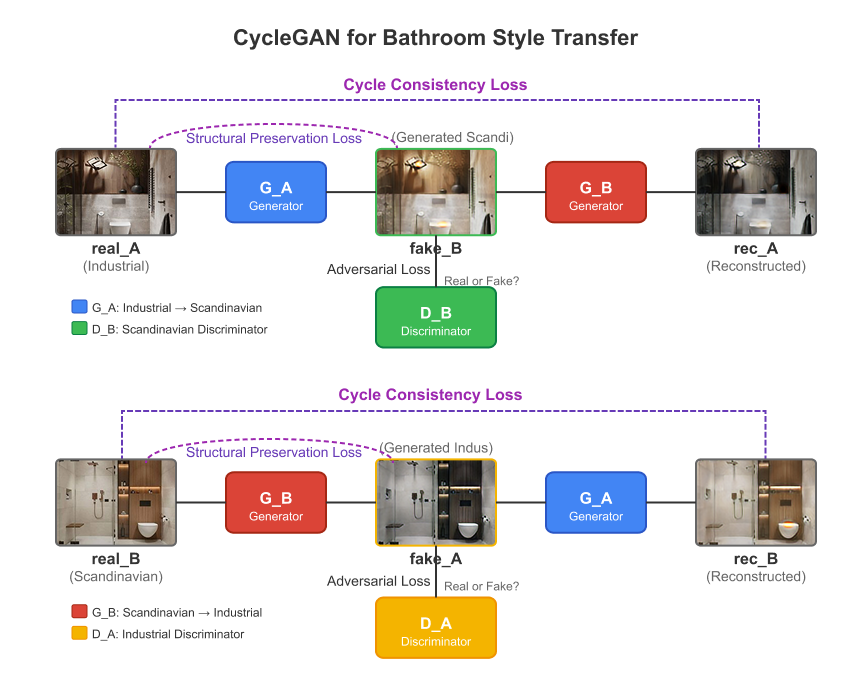
\includegraphics[width=\textwidth]{cyclegan_architecture.pdf}
    \caption{Enhanced CycleGAN architecture for bathroom style transfer. The system includes two generators (G$_A$ transforms Industrial to Scandinavian, G$_B$ transforms Scandinavian to Industrial) and two discriminators (D$_A$ and D$_B$). Additional loss functions (cycle consistency and structural preservation) help maintain both the content integrity and the distinctive stylistic elements.}
    \label{fig:architecture}
\end{figure}

\subsubsection{Enhanced Generator}

Our generator network uses a ResNet-based architecture with improvements for interior design style transfer:

\begin{itemize}
    \item Initial reflection padding and 7×7 convolution to preserve edge information, which is critical for maintaining bathroom structural elements
    \item Two downsampling layers with stride-2 convolutions and instance normalization
    \item Nine residual blocks for feature transformation while maintaining spatial information
    \item Improved upsampling using bilinear interpolation followed by 3×3 convolutions to reduce checkerboard artifacts common in transpose convolutions
    \item Final reflection padding and 7×7 convolution with Tanh activation
\end{itemize}

The dual generator structure allows us to create both Industrial→Scandinavian (G$_A$) and Scandinavian→Industrial (G$_B$) transformations. This bidirectionality enables cycle consistency training without requiring paired images.

\subsubsection{Multi-scale Discriminator}

To better capture both global structure and local details, we implemented a multi-scale discriminator that operates at two resolutions:

\begin{itemize}
    \item Full-resolution discriminator for capturing overall image coherence and stylistic patterns
    \item Half-resolution discriminator for focusing on larger-scale features (like layout and fixtures)
    \item Each discriminator uses a PatchGAN architecture with spectral normalization for training stability
\end{itemize}

This multi-scale approach helps the model better distinguish between industrial and scandinavian styles while maintaining structural coherence. For example, the full-resolution discriminator might focus on detailed textures like tile patterns or fixture finishes, while the half-resolution discriminator captures more general properties like color schemes and spatial arrangements.

\subsubsection{Perceptual Network}

For our structural preservation loss, we incorporated a perceptual network based on pre-trained VGG19 features. This network extracts features at three different depths, allowing us to capture different levels of structural information:

\begin{itemize}
    \item Low-level features (edges, textures) from early layers, which help preserve basic elements like walls and fixtures
    \item Mid-level features (patterns, local structures) from middle layers, capturing bathroom fixtures and their arrangement
    \item High-level features (spatial arrangements) from deeper layers, representing overall bathroom layout
\end{itemize}

By weighting these feature levels differently in our loss function (with higher weight on low and mid-level features), we encourage the model to preserve structural elements while still allowing stylistic changes appropriate for the target domain. This is especially important for bathroom style transfer, where we want to maintain the layout and fixtures while changing decorative elements to match either industrial or scandinavian design aesthetics.

\subsection{Loss Functions}

Our training objective combines several loss terms:

\begin{equation}
\mathcal{L} = \mathcal{L}_{GAN} + \lambda_{cycle}\mathcal{L}_{cycle} + \lambda_{id}\mathcal{L}_{id} + \lambda_{struct}\mathcal{L}_{struct}
\end{equation}

\subsubsection{Adversarial Loss}

We use the standard GAN loss with mean squared error (MSE) for stable training:

\begin{equation}
\mathcal{L}_{GAN}(G, D) = \mathbb{E}_{y}[(D(y) - 1)^2] + \mathbb{E}_{x}[D(G(x))^2]
\end{equation}

\subsubsection{Cycle Consistency Loss}

To ensure that the transformed images can be mapped back to their original versions:

\begin{equation}
\mathcal{L}_{cycle} = \mathbb{E}_{x}[||G_B(G_A(x)) - x||_1] + \mathbb{E}_{y}[||G_A(G_B(y)) - y||_1]
\end{equation}

\subsubsection{Identity Loss}

To encourage color preservation when appropriate:

\begin{equation}
\mathcal{L}_{id} = \mathbb{E}_{x}[||G_B(x) - x||_1] + \mathbb{E}_{y}[||G_A(y) - y||_1]
\end{equation}

\subsubsection{Structural Preservation Loss}

Our key innovation is a structural preservation loss that helps maintain architectural elements while changing style:

\begin{equation}
\mathcal{L}_{struct} = \sum_{i=1}^{3} w_i \cdot ||F_i(G_A(x)) - F_i(x)||_1 + \sum_{i=1}^{3} w_i \cdot ||F_i(G_B(y)) - F_i(y)||_1
\end{equation}

where $F_i$ represents the feature maps from the $i$-th layer of the perceptual network, and $w_i$ are weights decreasing with depth to allow style changes while preserving structure.

\section{Implementation}

\subsection{System Overview}

We implemented our system in Python using PyTorch as the deep learning framework. The codebase is organized into several key components:

\begin{itemize}
    \item \texttt{data\_preparation.py}: Dataset loading, preprocessing, and splitting
    \item \texttt{train.py}: Training script with Weights \& Biases integration
    \item \texttt{evaluate.py}: Evaluation metrics computation (LPIPS, FID)
    \item \texttt{inference.py}: Style transfer application to new images
    \item \texttt{models/}: Neural network architecture implementation
    \item \texttt{utils.py}: Utility functions for image processing
\end{itemize}

\subsection{Training Process}

We trained our model using the following hyperparameters:

\begin{itemize}
    \item Batch size: 4
    \item Learning rate: 0.0002 with Adam optimizer ($\beta_1=0.5$, $\beta_2=0.999$)
    \item Training epochs: 100
    \item Image size: 256×256
    \item Loss weights: $\lambda_{cycle}=10.0$, $\lambda_{id}=0.5$, $\lambda_{struct}=10.0$
\end{itemize}

The training process included several strategies for stability:
\begin{itemize}
    \item Learning rate decay using a step scheduler (half the rate every 30 epochs)
    \item Image buffer for discriminator training to reduce oscillation
    \item Spectral normalization in the discriminator
\end{itemize}

We used Weights \& Biases for experiment tracking, allowing us to monitor loss curves, learning rates, and generated samples throughout training.

\subsection{Evaluation Metrics}

We evaluated our model using two complementary metrics:

\begin{itemize}
    \item \textbf{LPIPS} (Learned Perceptual Image Patch Similarity): Measures perceptual similarity between images, used to evaluate both cycle consistency (how well the original image is reconstructed after a full cycle) and structural preservation (how well structural elements are maintained)
    \item \textbf{FID} (Fréchet Inception Distance): Measures the distance between the feature distributions of real and generated images, providing an assessment of overall generation quality
\end{itemize}

\section{Experiments and Results}

% Placeholder for experiments and results
\textit{This section will be populated with actual experimental results once they are available. It will include:}

\begin{itemize}
    \item \textit{Visual examples of style transfer between different bathroom styles}
    \item \textit{Quantitative evaluation using LPIPS and FID metrics}
    \item \textit{Ablation studies examining the contribution of different architectural components}
    \item \textit{Comparison with baseline methods}
\end{itemize}

\section{Discussion}

% Placeholder for discussion
\textit{This section will analyze the results and discuss:}

\begin{itemize}
    \item \textit{Strengths and limitations of our approach}
    \item \textit{Analysis of which bathroom styles were most challenging to transfer}
    \item \textit{The effectiveness of the structural preservation loss}
    \item \textit{Observed failure cases and potential improvements}
\end{itemize}

\section{Conclusion and Future Work}

In this paper, we presented a deep learning approach for bathroom interior design style transfer using an enhanced CycleGAN architecture. Our system can transform bathroom images between five different design styles while preserving structural elements. The key innovations include a multi-scale discriminator architecture and a structural preservation loss function specifically designed for interior spaces.

% Placeholder for specific conclusions
\textit{This section will be expanded with concrete conclusions based on experimental results.}

Future work could explore several promising directions:

\begin{itemize}
    \item Extending the approach to other room types beyond bathrooms
    \item Incorporating semantic segmentation to better preserve specific elements
    \item Developing controllable style transfer with adjustable intensity
    \item Exploring real-time implementation for interactive applications
\end{itemize}


% ==============================================================================

\bibliographystyle{unsrt}
\bibliography{bibliography.bib}

\end{document}